\documentclass[]{article}
\usepackage{amsmath}
\usepackage{amsfonts}
\usepackage{amssymb}
\usepackage{hyperref}
\usepackage{gensymb}
\usepackage{graphicx}
\usepackage{svg}
\usepackage{bbding}
\usepackage{mathtools}
\usepackage{centernot} % not parallel, etc.
\usepackage{lmodern}
\usepackage{morewrites}
\usepackage{xcolor,sectsty} % colorful sections
\usepackage[left=10mm, top=10mm, right=10mm, bottom=20mm, nohead]{geometry}
%\usepackage{bigints}
\usepackage{dsfont} %mathbb 1
\usepackage{esint} % beatiful integrals


\DeclareFontFamily{OMX}{lmex}{}
\DeclareFontShape{OMX}{lmex}{m}{n}{<-> lmex10}{}


%colors of sections
\definecolor{secfont}{RGB}{46,116,181}
\definecolor{subfont}{RGB}{146,23,57}
\definecolor{parfont}{RGB}{19,127,43}
\definecolor{subparfont}{RGB}{7,11,100}

\subsectionfont{\color{subfont}}
\sectionfont{\color{secfont}}
\paragraphfont{\color{parfont}}
\subparagraphfont{\color{subparfont}}

%\usepackage{babel}[english]
%opening
\title{104030 - Introduction to Partial Differential Equations}
\author{Gershon Velinski}

\parindent=0em
\begin{document}


\maketitle

\begin{abstract}

\end{abstract}

%\tableofcontents
\section{Introduction}
\paragraph{PDE}
In PDE, the solution is a function of a couple of variables $u(x_1, x_2, \dots x_m)$ such that:
$$F(x_1, x_2, \dots x_m, u_{x_1}, u_{x_2}, \dots, , u_{x_m}, u_{x_1x_1}, \dots) = 0$$
Notation is 
$$u_{x_i} = \frac{\partial u}{\partial x_i}$$
Usually $m=2$. For example
$$F(x_1,x_2, u, u_{x_1}, u_{x_2}, u_{x_1x_1}, u_{x_2x_2}, u_{x_1x_0}) = 0$$
Is PDE of two variables of order 2.
\paragraph{Linear PDE}
PDE is linear if $F$ is linear in $u$ and its derivatives. First order linear PDE is
$$F(x_1,x_2, u, u_{x_1}, u_{x_2}) = a(x_1,x_2)u_{x_1} + b(x_1,x_2)u_{x_2} + c(x_1,x_2)u + d(x_1,x_2) = 0$$
Second order linear PDE is
\begin{align*}
F(x_1,x_2, u, u_{x_1}, u_{x_2}, u_{x_1x_1}, u_{x_1x_2}, u_{x_2x_2}) =\\= A(x_1,x_2) u_{x_1x_1} + B(x_1,x_2) u_{x_1x_2} + C(x_1,x_2) u_{x_2x_2} + a(x_1,x_2)u_{x_1} + b(x_1,x_2)u_{x_2} + c(x_1,x_2)u + d(x_1,x_2) = 0
\end{align*}
\paragraph{Quasilinear PDE}
Quasilinear PDE is linear only in highest order derivative. First order quasilinear PDE:
$$F(x_1,x_2, u, u_{x_1}, u_{x_2}) = a(x_1,x_2, u)u_{x_1} + b(x_1,x_2, u)u_{x_2} + c(x_1,x_2, u) = 0$$
And second order one:
\begin{align*}
F(x_1,x_2, u, u_{x_1}, u_{x_2}, u_{x_1x_1}, u_{x_1x_2}, u_{x_2x_2}) =\\= A(x_1,x_2, u, u_{x_1}, u_{x_2}) u_{x_1x_1} + B(x_1,x_2, u, u_{x_1}, u_{x_2}) u_{x_1x_2} + C(x_1,x_2, u, u_{x_1}, u_{x_2}) u_{x_2x_2} + g(x_1,x_2, u, u_{x_1}, u_{x_2}) = 0
\end{align*}

For homogeneous linear PDE solution always exist. In addition, if $u_1$, $u_2$, then any linear combination of those $\lambda_1 u_1 + \lambda_2 u_2$ will also be a solution. Thus set of solutions of linear homogeneous PDE is vector space.

\paragraph{Autonomous PDE } If $F$ is independent on $x_i$, then if $u(x_1, \dots, x_i, \dots, x_m)$ is solution then $u(x_1, \dots, x_i+\lambda, \dots x_m)$ is solution too. 

In particular if $u$ is independent on all $x_i$, then $u(x_1+\lambda_1, \dots, x_i+\lambda_i, \dots, x_m+\lambda_m)$.

\subsection{Wave equation}
$$u_{tt} - c^2 u_{xx} = 0$$
Solution describes movement of wave.

Lets start ODE describing harmonic oscillator, would be
$$m \frac{d^2x}{dt^2} = k(x - x_0)$$

Now suppose that we have $N$ such masses and positionn of mass is $\bar{x}_i = x_i+u(x_i, t)$, where $u$ is displacement of mass and $x_i - x_{i-1} = \Delta$. Then the position of mass is described as
$$\frac{\partial \bar{x}_i}{\partial t^2} = m\frac{\partial^2 }{\partial t^2}u(x_i,t) = k(\bar{x}_{i+1}-\bar{x}_i)+k(\bar{x}_{i}-\bar{x}_{i-1})$$
Thus
$$m\frac{d}{dt^2}u(x,t) = k \left[ u(x_{i+1},t) - 2u(x_i,t) + u(x_{i-1},t) \right]$$
In limit $\Delta \to 0$:
$$\frac{d}{dt^2}u(x,t) = c^2\frac{d}{dx^2}u(x,t)$$
Where
$$c^2 = \lim_{\Delta \to 0} \frac{\Delta^2 k_\Delta}{m_\Delta} $$
\paragraph{Possible solutions}
For each function $f$ in $\mathcal{C}^2$, $u=f(x-ct)$ is a solution of wave equation:
$$\begin{cases}
u_{xx} = f''(x-ct)\\
u_{tt} = c^2 f''(x-ct)
\end{cases}$$

This solution is moving wave, because it moves along $x$ axis with constant velocity $c$. Since $c$ can be negative too, we have solution
$$u(x,t) = f(x+ct) + g(x-ct)$$
\subsection{Heat equation}
$$\frac{\partial u}{\partial t} = k \frac{\partial^2 u}{\partial x^2} $$
Here, $u$ means amount of heat in point $x$ at time $t$.

Amount of heat in interval $[a,b]$ is
$$Q(t) = \int_a^b u(x,t) dx$$
And heat flux in point $x$ at time $t$ is $k\frac{\partial u}{\partial x}$

Then flux out of interval is
$$\frac{dQ}{dt} = k\frac{\partial u}{\partial x}(b,t) - k\frac{\partial u}{\partial x}(a,t)$$
Thus
$$\int_a^b \frac{\partial }{\partial t}u(x,t) dx  = k\frac{\partial u}{\partial x}(b,t) - k\frac{\partial u}{\partial x}(a,t)$$
In limit $b\to a$ we get
$$\frac{\partial u}{\partial t} = k \frac{\partial^2 u}{\partial x^2} $$

\paragraph{Example solution}
$$u(x,t) = e^{-kst} \sin (\sqrt{s} x)$$
for some parameter $s$. Here we also can add some constant to $x$ and acquire additional solution:
$$U(x,t) = e^{-kst} \sin (\sqrt{s} (x+\lambda)) = \cos (\sqrt{s} \lambda ) e^{-kst} \sin (\sqrt{s} x) +  \sin (\sqrt{s} \lambda ) e^{-kst} \cos (\sqrt{s} x)$$
Thus
$$w(x,t) =  e^{-kst} \cos (\sqrt{s} x)$$
is solution too.
\subsection{Diffusion equation}
Suppose
$u(x_1,x_2,x_3,t)$ describes concentration of material in space. From continuity:
$$\frac{\partial u}{\partial t} + \vec{\nabla} \cdot (\vec{v} u) = 0$$
$$\frac{\partial u}{\partial t} +\frac{\partial }{\partial x_1} (\vec{v} u) +\frac{\partial }{\partial x_2} (\vec{v} u) +\frac{\partial }{\partial x_3} (\vec{v} u) = 0$$
for some vector field $v$ independent on $u$.
\subsection{Elliptic PDEs}
\paragraph{Laplace equation}
$$\Delta u = \frac{\partial^2 u}{\partial x_1^2} + \frac{\partial^2 u}{\partial x_2^2} = 0$$
\paragraph{Poisson equation}
$$\Delta u = f(x_1,x_2)$$
\section{First-order PDE}
$$\frac{\partial u}{\partial t} + c\frac{\partial u}{\partial x} = 0$$
We can easily guess solution similarly to wave equation: $u(x,t) = f(x-ct)$ for some differentiable $f$. 

Suppose we have initial conditions $u(x,0)= u_0(x)$. Is it determines uniquely a solution of equation? Obviously, $u(x,t) = u_0(x-ct)$ is a solution.

Lets show it's unique. Take a look at parametrization $x(t) = s_1 + ct$.
$$\frac{d}{dt} u(x(t),t) = c\frac{\partial u}{\partial x}(x(t),t) + \frac{\partial u}{\partial t}(x(t),t) = 0$$ 
Thus $u$ is constant on every line of form $x(t)=s+ct$. Such lines are called characteristic curves or just characteristics. Thus if we know a value of $u$ in some point on a line, we know it on the whole line.

\paragraph{} Is it possible to find a solution if we are given initial conditions for some curve $x(t)$ for $t \in [a,b]$. So we want to find a solution such that the surface of solution comprises a given curve in 3D.

The solution exists if the curve of initial conditions doesn't merges with characteristic line, we have a unique solution. If it does, either there is no solution, or there are infinite number of solution.

\subsection{Quasilinear first-order equations}
$$a(x,y,u)u_x + b(x,y,u)u_y = c(x,y,u)$$
where $a,b,c$ are continuously differentiable in some neighborhood of point $(x_0,y_0,z_0)$.

Take a look at
$$f(x,y,z) = z - u(x,y)$$
$$\nabla f = \left(-\frac{\partial u}{\partial x},-\frac{\partial u}{\partial y},1\right)$$
and
$$\nabla f \cdot (a,b,c) = -a\frac{\partial u}{\partial x} -b\frac{\partial u}{\partial y}+c  = 0$$
Thus vector $(a,b,c) $ is tangent to solution surface.

Now define curve such that
$$\begin{cases}
\frac{dx}{dt} = a(x(t), y(t), z(t))\\
\frac{dy}{dt} = b(x(t), y(t), z(t))\\
\frac{dz}{dt} = c(x(t), y(t), z(t))
\end{cases}$$
The curve $\left(x(t), y(t), z(t)\right)$ is characteristic curve of PDE.

If there is no dependence on $z$ (i.e.\ equation is linear) we can take a look on 2-dimensional curve in xy-plane.

\paragraph{Theorem}
If characteristic curve intersects solution surface of quasilinear first-order PDE at some point, it is contained in the surface.
\subparagraph{Proof}
Let $\left(x(t), y(t), z(t)\right)$ characteristic curve of PDE and suppose for some $t_0$ 
$$u(x(t_0), y(t_0)) = z(t_0)$$
Define 
$$w(t) = z(t) - u(x(t),y(t))$$
Note that $w(t_0) = 0$.  Now
\begin{align*}
G\big(x(t),y(t), w(t)\big) = \frac{dw}{dt} = \frac{dz}{dt} - \frac{\partial u}{\partial x}\big(x(t), y(t)\big) \frac{dx}{dt}-  \frac{\partial u}{\partial y}\big(x(t), y(t)\big) \frac{dy}{dt} = c\bigg(x(t),y(t),w(t)+u\big(x(t),y(t)\big)\bigg) -\\- \frac{\partial u}{\partial x}\big(x(t), y(t)\big) a\bigg(x(t),y(t),w(t)+u\big(x(t),y(t)\big)\bigg) - \frac{\partial u}{\partial y}\big(x(t), y(t)\big) b\bigg(x(t),y(t),w(t)+u\big(x(t),y(t)\big))\bigg)
\end{align*}
If we substitute $w=0$, we get
$$G\big(x(t),y(t), 0\big) = c\big(x(t),y(t),u\big(x(t),y(t)\big)\big) -\frac{\partial u}{\partial x}(x(t), y(t)) a\big(x(t),y(t),u\big(x(t),y(t)\big)\big) - \frac{\partial u}{\partial y}(x(t), y(t)) b\big(x(t),y(t),u\big(x(t),y(t)\big))\big)=0$$
That means that $w=0$ is a solution of ODE, and since $a,b,c\in \mathcal{C}^1$, te solution is unique, i.e. $w=0$ is the only solution, and thus characteristic curve is contained in the solution surface.
\subsection{Existence and uniquness theorem for first-order quasilinear PDE}
\paragraph{Existence and uniquness theorem for first-order quasilinear PDE}
Suppose we have initial curve $\Gamma(s) = \left(\bar{x}(s), \bar{y}(s), \bar{z}(s) \right)$ which around some point $s_0$ is continuously differentiable. Suppose also
$$a(x_0,y_0,z_0) \dot{\bar{y}}(s_0) - b(x_0,y_0,z_0) \dot{\bar{x}}(s_0) \neq 0$$
(transversality condition). 

Then in neighborhood of $s_0$ exists unique solution of PDE.

\subparagraph{Proof}
Define functions $x(s,t)$, $y(s,t)$, $z(s,t)$ around $(s_0,0)$  such that
$$\begin{cases}
x(s,0) = \bar{x}(s)\\
y(s,0) = \bar{y}(s)\\
z(s,0) = \bar{z}(s)\\
\end{cases}$$
and
$$\begin{cases}
\frac{\partial x}{\partial t} = a\big(x(s,t), y(s,t), z(s,t)\big)\\
\frac{\partial y}{\partial t} = b\big(x(s,t), y(s,t), z(s,t)\big)\\
\frac{\partial z}{\partial t} = c\big(x(s,t), y(s,t), z(s,t)\big)
\end{cases}$$
From uniquness and existance of ODE, exists unique solution $(x,y,z)$ in neighbourhood of $s_0$.

Lets try to find $s$, $t$, as a function of $x$,$y$. It is possible if conditions of inverse function theorem are fulfilled, i.e.\
$$\begin{vmatrix}
\frac{\partial x}{\partial s}&\frac{\partial x}{\partial t}\\
\frac{\partial y}{\partial s}&\frac{\partial y}{\partial t}\\
\end{vmatrix}\neq 0$$
in $(s_0,0)$.

Now define $u(x,y) = z\big(s(x,y), t(x,y)\big)$.
\begin{align*}
a\frac{\partial u}{\partial x}+b\frac{\partial u}{\partial y} = a\left[\frac{\partial z}{\partial s}\frac{\partial s}{\partial x}+\frac{\partial z}{\partial t}\frac{\partial t}{\partial x}\right]+b\left[\frac{\partial z}{\partial s}\frac{\partial s}{\partial y}+\frac{\partial z}{\partial t}\frac{\partial t}{\partial y}\right] = \frac{\partial z}{\partial t} \left[a\frac{\partial t}{\partial x} + b\frac{\partial t}{\partial y}\right] + \frac{\partial z}{\partial s} \left[a\frac{\partial s}{\partial x} + b\frac{\partial s}{\partial y}\right] =\\= \frac{\partial z}{\partial t} \underbrace{\left[\frac{\partial x}{\partial t}\frac{\partial t}{\partial x} + \frac{\partial y}{\partial t}\frac{\partial t}{\partial y}\right]}_{\frac{dt}{dt}} + \frac{\partial z}{\partial s} \underbrace{ \left[\frac{\partial x}{\partial t}\frac{\partial s}{\partial x} + \frac{\partial y}{\partial t}\frac{\partial s}{\partial y}\right]}_{\frac{ds}{dt}} = \frac{\partial s}{\partial t} = c
\end{align*}

If crossing conditions are not fulfilled we have a couple of options:
\begin{itemize}
	\item If initial curve is characteristic curve, we have infinite number of solutions.
	\item If initial curve is not characteristic curve, but their projection on $xy$-plane is same, we have no solution, since each solution includes characteristic curve.
\end{itemize}

In other cases, if for example initial curve is tangent to characteristic curve and their projection on $xy$-plane are different, there are different possibilities.

\paragraph{Example}
$$yu_x - xu_y = 0$$
with initial curve $(s,0,h(s))$ and $0<\alpha\leq s\leq \beta$
\subparagraph{Solution}
$$\begin{cases}
\dot{x} = y\\
\dot{y} = -x\\
\dot{z} = 0
\end{cases} \Rightarrow \begin{cases}
\ddot{x} = -x\\
\ddot{y} = -y\\
\dot{z} = 0
\end{cases} \Rightarrow \begin{cases}
x = A(s)\sin(t)+B(s)\cos(t)\\
y = A(s)\cos(t)-B(s)\sin(t)\\
z = c
\end{cases}$$
Now from initial curve
$$A(s)= s \quad B(s) = 0$$
$$ \begin{cases}
x = s\cos(t)\\
y = -s\sin(t)\\
z = h(s)
\end{cases}$$
Now we want to find $s$, $t$ as a function of $x$,$y$:
$$x^2+y^2 = s^2 \Rightarrow s = \sqrt{x^2+y^2}$$
$$u(x,y)  = h\left(\sqrt{x^2+y^2}\right)$$
Note that characteristic curves are rings.

\paragraph{Example}
$$yu_x - xu_y = u$$
with initial curve $(s,0,h(s))$ and $0<\alpha\leq s\leq \beta$
\subparagraph{Solution}
$$\begin{cases}
\dot{x} = y\\
\dot{y} = -x\\
\dot{z} = u
\end{cases} \Rightarrow \begin{cases}
\ddot{x} = -x\\
\ddot{y} = -y\\
z = C(s)e^t
\end{cases} \Rightarrow \begin{cases}
x = A(s)\sin(t)+B(s)\cos(t)\\
y = A(s)\cos(t)-B(s)\sin(t)\\
z = C(s)e^t
\end{cases}$$
Now from initial curve
$$A(s)= s \quad B(s) = 0$$
$$ \begin{cases}
x = s\cos(t)\\
y = -s\sin(t)\\
z = h(s)e^t
\end{cases}$$
Now we want to find $s$, $t$ as a function of $x$,$y$:
$$x^2+y^2 = s^2 \Rightarrow s = \sqrt{x^2+y^2}$$
And
$$\tan t  = -\frac{y}{x} \Rightarrow t = \arctan \left(-\frac{y}{x}\right)$$
$$u(x,y)  = h\left(\sqrt{x^2+y^2}\right)e^{ \arctan \left(-\frac{y}{x}\right)}$$


\subsection{Burgers' equation}
$$u_y + uu_x = 0$$
(which is partial case of equation of form $$\pdv{u}{y} + \pdv{ y} F(u) = 0$$ for $F=\frac{1}{2}u^2$)

Note that $$\frac{u_y}{u_x} = -u \Rightarrow \dv{x}{y} = - u \Rightarrow u = -\dv{x}{y}$$
Here $y$ denotes time.

To solve it, we take integral:
$$\int_a^b \left[ \pdv{ u(x,y)}{y} + \pdv {x} F(u(x,y))\right] \dd{x} = 0$$
$$\pdv{y} \underbrace{\int_a^b u \dd{x}}_{Q(y)}  + F\Big(u(b,y)\Big) - F\Big(u(a,y)\Big) = 0$$
$$\dv{Q}{y} = F\Big(u(a,y)\Big) - F\Big(u(b,y)\Big)$$

Now as for any quasilinear PDE:
$$\begin{cases}
\dot{x}= z\\\dot{y} = 1\\\dot{z}= 0
\end{cases} \Rightarrow \begin{cases}
x= c_2 t + c_3\\y = t + c_1\\\dot{z}= c_2
\end{cases} $$
For initial conditions $\Big(s,0,h(s)\Big)$:
$$ \begin{cases}
x= h(s) t + s\\y = t \\z= h(s)
\end{cases} $$
Now 
$$s=x-yu \Rightarrow u = h(x-yu)$$
Checking transversality condition:
$$\dv{\bar{x}}{s} \cdot 1 - \dv{\bar{y}}{s} \cdot h(s) = 1 \neq 0$$  


Since
$$\pdv{u}{x} = h'(x-yu) \cdot \left(1 - y\pdv{u}{x} \right)$$
$$\pdv{u}{x} = \frac{h'(x-yu)}{1+h'(x-yu) \cdot y} $$
even if we start from $\mathcal{C}^\infty$ function we can get $1+h'(x-yu) \cdot y = 0$ and thus undefined derivative.

Geometrically, the slope of projections of characteristic curves is equal to $h(s)$ thus they can cross in some point.

\paragraph{Weak solutions}
We define a weak solution of equation, function $u$  fulfilling the equation:
$$\forall a,b \quad \pdv{y} u(x,y) \dd{x} + F\Big(u(b,y)\Big)-F\Big(u(a,y)\Big) = 0$$

Intuitively, $F$ is flux, and $u$ is density, thus change in number of particles (integral) is difference between particles going in and out.

Suppose for solution $u(x,y)$ exists curve of non-continuousness $\gamma$, i.e, $u$ is not continuous in each point of curve:
$$u(y) = \begin{cases}
u^+(y) & y < \gamma(y)\\
u^-(y) & y > \gamma(y)
\end{cases}$$

$$Q_{a,b}(y) = \int_a^b u(x,y) \dd{x} = \int_a^{\gamma(y)} u^+(x,y) \dd{x} + \int_{\gamma(y)}^{b} u^-(x,y) \dd{x}$$ 
\begin{align*}
\pdv{Q}{y} = \int_a^{\gamma(y)} \pdv{u^+(x,y)}{y} \dd{x} + u^+(x,\gamma(y)) \cdot \gamma'(y) + \int_{\gamma(y)}^{b} \pdv{u^-(x,y)}{y} \dd{x}-  u^-(x,\gamma(y)) \cdot \gamma'(y) =\\= - \int_{a}^{\gamma(y)}  \dv{F(u^+)}{x} \dd{x} - \int_{\gamma(y)}^{b} \dv{F(u^-)}{x} \dd{x} + \gamma'(y) \left[ u^+\Big(x,\gamma(y)\Big) -  u^-\Big(x,\gamma(y)\Big) \right] =\\= -\left[F\Big(u^+\big(\gamma(y),y\big)\Big)-F\Big(u^+(a,y)\Big)\right]-\left[F\Big(u^-(b,y)\Big)-F\Big(u^+\big(\gamma(y),y\big)\Big)\right] + \gamma'(y) \left[ u^+\Big(x,\gamma(y)\Big) -  u^-\Big(x,\gamma(y)\Big)  \right]
\end{align*}
Meaning
\begin{align*}
-\bigg[F\Big(u^+\big(\gamma(y),y\big)\Big)-F(u^+(a,y))\bigg]-\bigg[F\Big(u^-(b,y)\Big)-F\Big(u^+\big(\gamma(y),y\big)\Big)\bigg] + \gamma'(y) \bigg[ u^+(x,\gamma(y)) -  u^-(x,\gamma(y))  \bigg] =\\= F\Big(u^-(a,y)\Big) - F\Big(u^+(b,y)\Big) 
\end{align*}
$$ $$
$$  \gamma'(y) \bigg[ u^+\Big(x,\gamma(y)\Big) -  u^-\Big(x,\gamma(y)\Big)  \bigg] = F\Big(u^+\big(\gamma(y),y\big)\Big) - F\Big(u^-\big(\gamma(y),y\big)\Big)  $$
$$\gamma' = \frac{ F\Big(u^+(\gamma(y),y)\Big) - F\Big(u^-\big(\gamma(y),y\big)\Big)}{u^+\big(x,\gamma(y)\big) -  u^-\big(x,\gamma(y)\big) }$$
This equation is called Rankine–Hugoniot conditions.
If $F(u) = \frac{1}{2}u^2$, we get $\gamma'(y) = \frac{1}{2}\left(u^+ + u^-\right)$

\paragraph{Example}
Suppose we have initial conditions $u(x,0) = h(x)$ for
$$h(x) = \begin{cases}
1 & x < 0\\
0 & x> \alpha\\
1-\frac{x}{\alpha} & 0\leq x \leq \alpha
\end{cases}$$

For $0<y<1$ we have a triangle $\Delta$ ($0<x<\alpha$ and $y < \frac{x}{\alpha}$) for which there is intersection of two solution:

\begin{center}
	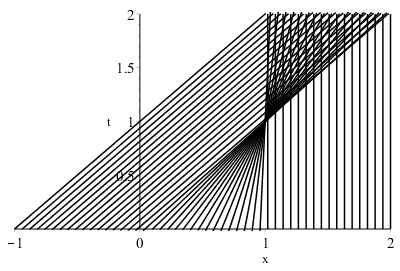
\includegraphics[width=0.5\linewidth]{./lect2/p2.png}
\end{center}

In point $x,y$ we have slope $u(x,y)$ thus the charecteristic curve crosses $x$-axis at $x_0 = x-uy$ and from initial conditions, $u=1-\frac{x_0}{\alpha}$. Thus
$$u=1-\frac{x-uy}{\alpha}$$
$$\alpha u=\alpha-x+uy$$
$$(\alpha-y) u=\alpha-x$$
Acquiring
$$u = \frac{x-\alpha}{y-\alpha}$$
And now for $y>1$ from Rankine–Hugoniot conditions
$$u(x,y) = \begin{cases}
1 & x<\alpha + \frac{1}{2} (y-\alpha)\\
0 & x>\alpha + \frac{1}{2} (y-\alpha)\\
\end{cases}$$
Such a solution is called a shock wave.

\begin{center}
	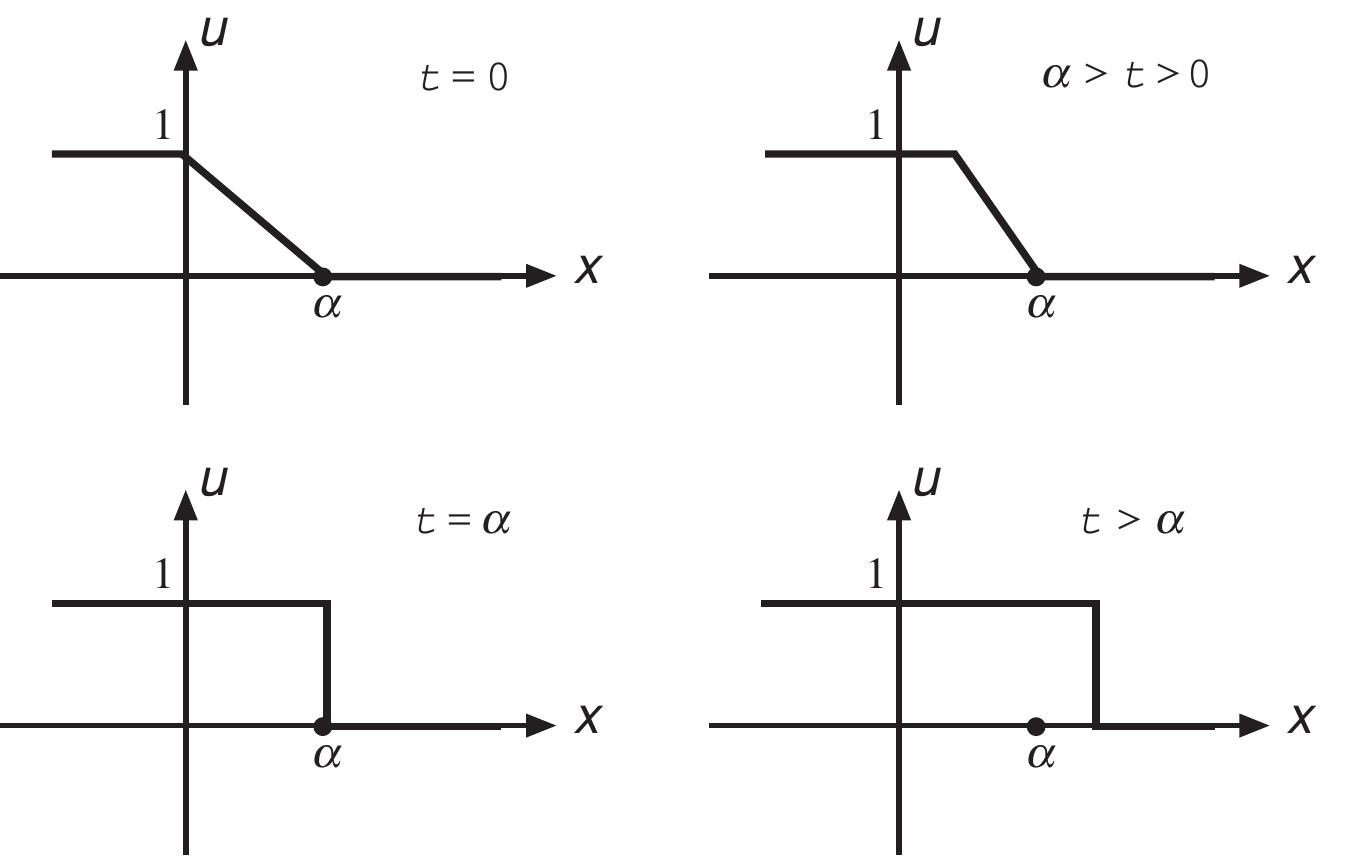
\includegraphics[width=0.7\linewidth]{./lect2/p1.png}
\end{center}

\paragraph{Example}
For
$$h(x) = \begin{cases}
0 & x> \alpha\\
1 & x < 0\\
\frac{x}{\alpha} & 0\leq x \leq \alpha
\end{cases}$$

Now there is no place where characteristic curves meet

\begin{center}
	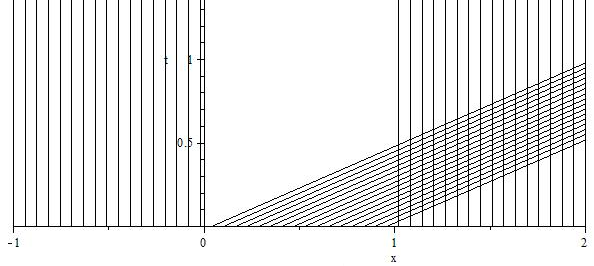
\includegraphics[width=0.7\linewidth]{./lect2/p3.png}
\end{center}

In the region without characteristic curves ($0\leq x\leq y$) we get the following: the solution starts from some  point $x_0 = x-uy$, and similarly to the previous case, from initial conditions,
$$u=\frac{x}{\alpha +y}$$


\begin{center}
	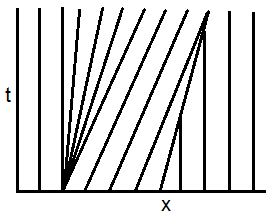
\includegraphics[width=0.3\linewidth]{./lect2/p4.png}
\end{center}

\paragraph{What happens if $\alpha \to 0$?}
We get $u=\frac{x}{y}$ for $0\leq x \leq y$. We acquired rarefaction wave - starting from something non-continuous we got continuous solution. This is weak solution.

However, also shock wave along $y=x$ is also solution of initial conditions. This solution is worse, because shock wave loses information, which means we cant reproduce the solution for some $y<y_0$ even if I know the values for $y=y_0$.
\paragraph{Entory principle}
Weak solution is unique if characteristic curves meet shock wave from direction of increasing time. 


\subsection{Fully non-linear equations}
\paragraph{Hamilton-Jacoby equation}
$$u_x^2+u_y^2=1$$
Can we generalize the method of solution of quasilinear equations to fully non-linear equations? The answer is yes. 
We have some $$F(x,y,u,u_x,u_y) = 0$$. In our case $$F(x,y,u,p,q) = p^2+q^2-1$$

Characteristic equations:
$$\begin{cases}
\dv{x}{t} = \pdv{F}{p}\\
\dv{y}{t} = \pdv{F}{q}\\
\dv{z}{t} = p\pdv{F}{p}+q\pdv{F}{q}\\
\dv{p}{t} = -\pdv{F}{x}+p\pdv{F}{z}\\
\dv{q}{t} = -\pdv{F}{y}+q\pdv{F}{z}\\
\end{cases}$$


Suppose we have initial curve $\Gamma = (\bar{x}(s), \bar{y}(s), \bar{z}(s))$

We need to find $\bar{p}$ and $\bar{q}$. We have two additional conditions:
$$F(x,y,u,u_x,u_y) = 0$$
also
$$u(\bar{x}(s), \bar{y}(s)) = \bar{z}(s)$$
Differentiating by $s$
$$\pdv{u}{x}\dv{\bar{x}}{s}  + \pdv{u}{y}\dv{\bar{y}}{s} = \dv{\bar{z}}{s}$$
$$\bar{p}(s)\dv{\bar{x}}{s} + \bar{q}(s)\dv{\bar{y}}{s} = \dv{\bar{z}}{s}$$
Now we can find $p$ and $q$.

Back to our equation:
$$\begin{cases}
\dot{x} = 2p\\
\dot{y} = 2q\\
\dot{z} = 2(p^2+q^2)\\
\dot{p} = \dot{q} = 0
\end{cases}$$

In case we have initial curve with $u=0$, then characteristic curves are perpendicular to initial curve.  We get $u(x,y)$ equal to distance from initial curve, since absolute value of gradient of $u$ is $1$ due to equation.

If we have $u=\phi(s)$ on initial curve, we acquire
$$u(x,y) = \min (x-\bar{x}(s))^2 + (y-\bar{y}(s))^2 + \phi(s)$$

\paragraph{Higher dimension}
We can trivially extend quasilinear equations to more dimensions. In this case we have initial surface instead of curve.
\section{Wave equation}
$$u_{tt} -c^2u_{xx} = 0$$
More generally, any second order linear equation can be written as
$$a(x,y) u_{xx} + 2b(x,y) u_{xy} + c(x,y) u_{yy} + du_x + eu_y + fu = g$$

\paragraph{Definition}
Equation is called hyperbolic if $b^2-ac>0$, parabolic if  $b^2-ac=0$ and elliptic if  $b^2-ac<0$. Wave equation is hyperbolic in the whole space.

We want to simplify the equation: we are searching for $\xi(x,y)$ and $\eta(x,y)$ such that
$$\pdv{\eta}{x} \pdv{\xi}{y} - \pdv{\eta}{y} \pdv{\xi}{x} \neq 0$$
and solution $u(x,y) = w\big(\xi(x,y), \eta(x,y)\big)$.

Derivatives of $u$ are
$$u_y = w_\xi \xi_y + w_\eta \eta_y$$
$$u_{yy} = w_{\xi\xi} \xi_{y}^2 + w_{\xi\eta}\xi_y\eta_y + w_{\xi}\xi_{yy} + w_{\eta \xi}\eta_y\xi_y + w_{\eta\eta} \eta_{y}^2+ w_{\eta}\eta_{yy}  $$
$$u_{xy} =\pdv{x}\pdv{u}{y} = w_{\xi \xi} \xi_x\xi_y + w_{\xi\eta}\xi_y\eta_x + w_{\xi\eta}\xi_x\eta_y + w_{\eta \xi} \eta_x\eta_y + w_{\xi}\xi_{xy}+w_\eta\eta_{xy}$$

Now we can get equation of form
$$A(\xi,\eta) w_{\xi\xi} + 2B(\xi,\eta) w_{\xi\eta} + C(\xi,\eta) w_{\eta \xi} + D(\xi,\eta) w_{\eta\eta}+ F(\xi,\eta) = 0$$
If we can find variable substitution such that
$$A=C=0$$
Then, in case of $d=e=f=0$,
$$Bw_{\xi\eta} = 0$$
i.e.,
$$w(\xi,\eta) = f(\xi)+g(\eta)$$
\end{document}
